%Version 3.1 December 2024
% See section 11 of the User Manual for version history
%
%%%%%%%%%%%%%%%%%%%%%%%%%%%%%%%%%%%%%%%%%%%%%%%%%%%%%%%%%%%%%%%%%%%%%%
%%                                                                 %%
%% Please do not use \input{...} to include other tex files.       %%
%% Submit your LaTeX manuscript as one .tex document.              %%
%%                                                                 %%
%% All additional figures and files should be attached             %%
%% separately and not embedded in the \TeX\ document itself.       %%
%%                                                                 %%
%%%%%%%%%%%%%%%%%%%%%%%%%%%%%%%%%%%%%%%%%%%%%%%%%%%%%%%%%%%%%%%%%%%%%

%%\documentclass[referee,sn-basic]{sn-jnl}% referee option is meant for double line spacing

%%=======================================================%%
%% to print line numbers in the margin use lineno option %%
%%=======================================================%%

%%\documentclass[lineno,pdflatex,sn-basic]{sn-jnl}% Basic Springer Nature Reference Style/Chemistry Reference Style

%%=========================================================================================%%
%% the documentclass is set to pdflatex as default. You can delete it if not appropriate.  %%
%%=========================================================================================%%

%%\documentclass[sn-basic]{sn-jnl}% Basic Springer Nature Reference Style/Chemistry Reference Style

%%Note: the following reference styles support Namedate and Numbered referencing. By default the style follows the most common style. To switch between the options you can add or remove “Numbered” in the optional parenthesis. 
%%The option is available for: sn-basic.bst, sn-chicago.bst%  
 
%%\documentclass[pdflatex,sn-nature]{sn-jnl}% Style for submissions to Nature Portfolio journals
%%\documentclass[pdflatex,sn-basic]{sn-jnl}% Basic Springer Nature Reference Style/Chemistry Reference Style
%%\documentclass[pdflatex,sn-mathphys-num]{sn-jnl}% ESSE É O ORIGINALMath and Physical Sciences Numbered Reference Style
\documentclass[pdflatex,sn-mathphys-num,iicol]{sn-jnl}
%%\documentclass[pdflatex,sn-mathphys-ay]{sn-jnl}% Math and Physical Sciences Author Year Reference Style
%%\documentclass[pdflatex,sn-aps]{sn-jnl}% American Physical Society (APS) Reference Style
%%\documentclass[pdflatex,sn-vancouver-num]{sn-jnl}% Vancouver Numbered Reference Style
%%\documentclass[pdflatex,sn-vancouver-ay]{sn-jnl}% Vancouver Author Year Reference Style
%%\documentclass[pdflatex,sn-apa]{sn-jnl}% APA Reference Style
%%\documentclass[pdflatex,sn-chicago]{sn-jnl}% Chicago-based Humanities Reference Style

%%%% Standard Packages
%%<additional latex packages if required can be included here>

%%<additional latex packages if required can be included here>
\usepackage{graphicx}      % Gerenciamento de imagens (carregado primeiro)
\usepackage{float}         % Permite o uso do [H] para fixar figuras e tabelas
\usepackage[section]{placeins} % Impede flutuantes de passarem das seções
\usepackage{subcaption}    % Permite subfiguras (se der erro no seu template, comente esta linha)
\usepackage{multirow}      % Mesclar linhas em tabelas
\usepackage{amsmath,amssymb,amsfonts} % Pacotes matemáticos
\usepackage{amsthm}        % Teoremas matemáticos
\usepackage{mathrsfs}      % Fontes manuscritas matemáticas
\usepackage[title]{appendix} % Apêndices
\usepackage{xcolor}        % Cores no texto
\usepackage{textcomp}      % Caracteres especiais
\usepackage{manyfoot}      % Notas de rodapé avançadas
\usepackage{booktabs}      % Linhas profissionais para tabelas (\toprule, \midrule, \bottomrule)
\usepackage{algorithm}     % Ambientes de algoritmo
\usepackage{algorithmicx}
\usepackage{algpseudocode}
\usepackage{listings}      % Inclusão de códigos de programação
%%%%



%%%%%=============================================================================%%%%
%%%%  Remarks: This template is provided to aid authors with the preparation
%%%%  of original research articles intended for submission to journals published 
%%%%  by Springer Nature. The guidance has been prepared in partnership with 
%%%%  production teams to conform to Springer Nature technical requirements. 
%%%%  Editorial and presentation requirements differ among journal portfolios and 
%%%%  research disciplines. You may find sections in this template are irrelevant 
%%%%  to your work and are empowered to omit any such section if allowed by the 
%%%%  journal you intend to submit to. The submission guidelines and policies 
%%%%  of the journal take precedence. A detailed User Manual is available in the 
%%%%  template package for technical guidance.
%%%%%=============================================================================%%%%

%% as per the requirement new theorem styles can be included as shown below
\theoremstyle{thmstyleone}%
\newtheorem{theorem}{Theorem}%  meant for continuous numbers
%%\newtheorem{theorem}{Theorem}[section]% meant for sectionwise numbers
%% optional argument [theorem] produces theorem numbering sequence instead of independent numbers for Proposition
\newtheorem{proposition}[theorem]{Proposition}% 
%%\newtheorem{proposition}{Proposition}% to get separate numbers for theorem and proposition etc.

\theoremstyle{thmstyletwo}%
\newtheorem{example}{Example}%
\newtheorem{remark}{Remark}%

\theoremstyle{thmstylethree}%
\newtheorem{definition}{Definition}%

\raggedbottom
%%\unnumbered% uncomment this for unnumbered level heads

\begin{document}

\title[Article Title]{
Position Control of a Two-Propeller Aeropendulum: A Comparison Between Voltage and Current Actuation
}

%%=============================================================%%
%% GivenName	-> \fnm{Joergen W.}
%% Particle	-> \spfx{van der} -> surname prefix
%% FamilyName	-> \sur{Ploeg}
%% Suffix	-> \sfx{IV}
%% \author*[1,2]{\fnm{Joergen W.} \spfx{van der} \sur{Ploeg} 
%%  \sfx{IV}}\email{iauthor@gmail.com}
%%=============================================================%%

\author*[1,2]{\fnm{First} \sur{Author}}\email{iauthor@gmail.com}

\author[2,3]{\fnm{Second} \sur{Author}}\email{iiauthor@gmail.com}
\equalcont{These authors contributed equally to this work.}

\author[1,2]{\fnm{Third} \sur{Author}}\email{iiiauthor@gmail.com}
\equalcont{These authors contributed equally to this work.}

\affil*[1]{\orgdiv{Department}, \orgname{Organization}, \orgaddress{\street{Street}, \city{City}, \postcode{100190}, \state{State}, \country{Country}}}

\affil[2]{\orgdiv{Department}, \orgname{Organization}, \orgaddress{\street{Street}, \city{City}, \postcode{10587}, \state{State}, \country{Country}}}

\affil[3]{\orgdiv{Department}, \orgname{Organization}, \orgaddress{\street{Street}, \city{City}, \postcode{610101}, \state{State}, \country{Country}}}

%%==================================%%
%% Sample for unstructured abstract %%
%%==================================%%

\abstract{This paper presents the development and validation of a low-cost twin-rotor aeropendulum testbed to evaluate the impact of low-level actuation on aerospace control systems. Standard brushless propulsion units traditionally drive the plant via voltage signals (PWM), introducing severe dynamic non-linearities and thrust asymmetries. To address this, we propose and compare two low-level frameworks: a conventional equivalent voltage-driven scheme and a software-based virtual estimated current-loop. Both are benchmarked under classical PID and adaptive hybrid Fuzzy-PID controllers. Experimental results show that the virtual current loop successfully linearizes the actuation channel, providing superior dynamic damping and a drastic reduction in the control energy index (ISSC) compared to the voltage scheme. Under external disturbances, the current-driven paradigm demonstrates high robustness and steady-state precision. Furthermore, while the current-driven Fuzzy-PID achieves the best performance-to-energy trade-off at positive setpoints, the conventional PID with virtual current actuation proves to be the most balanced and reliable strategy at negative operating points.}
%%================================%%
%% Sample for structured abstract %%
%%================================%%

% \abstract{\textbf{Purpose:} The abstract serves both as a general introduction to the topic and as a brief, non-technical summary of the main results and their implications. The abstract must not include subheadings (unless expressly permitted in the journal's Instructions to Authors), equations or citations. As a guide the abstract should not exceed 200 words. Most journals do not set a hard limit however authors are advised to check the author instructions for the journal they are submitting to.
% 
% \textbf{Methods:} The abstract serves both as a general introduction to the topic and as a brief, non-technical summary of the main results and their implications. The abstract must not include subheadings (unless expressly permitted in the journal's Instructions to Authors), equations or citations. As a guide the abstract should not exceed 200 words. Most journals do not set a hard limit however authors are advised to check the author instructions for the journal they are submitting to.
% 
% \textbf{Results:} The abstract serves both as a general introduction to the topic and as a brief, non-technical summary of the main results and their implications. The abstract must not include subheadings (unless expressly permitted in the journal's Instructions to Authors), equations or citations. As a guide the abstract should not exceed 200 words. Most journals do not set a hard limit however authors are advised to check the author instructions for the journal they are submitting to.
% 
% \textbf{Conclusion:} The abstract serves both as a general introduction to the topic and as a brief, non-technical summary of the main results and their implications. The abstract must not include subheadings (unless expressly permitted in the journal's Instructions to Authors), equations or citations. As a guide the abstract should not exceed 200 words. Most journals do not set a hard limit however authors are advised to check the author instructions for the journal they are submitting to.}

\keywords{Aeropendulum, Actuation dynamics, Virtual current loop, Fuzzy-PID control, Energy efficiency.}

%%\pacs[JEL Classification]{D8, H51}

%%\pacs[MSC Classification]{35A01, 65L10, 65L12, 65L20, 65L70}

\maketitle

\section{Introduction}\label{sec1}

Control systems play a central role in the advancement of modern technologies by ensuring precision, stability, and operational efficiency even in the face of disturbances and severe dynamic conditions. However, translating abstract mathematical models encountered in academic settings into real-world solutions requires a rigorous alignment between theory and experimental validation—a connection that characterizes a persistent pedagogical and technical challenge in the development of new technologies. 
Aiming to mitigate this gap between academia and the practical demands of industry, recent investigations, such as those conducted by \citet{antunes2026improving}, propose restructuring technical learning through methodologies based on practical and interdisciplinary projects. This approach is grounded in the strategic use of didactic platforms and testbeds, which emerge as a fundamental link in control engineering by offering a safe, replicable, and low-cost environment to evaluate the performance of new algorithms before their effective transition to high-complexity applications.

Among the real-world applications requiring this high level of technical rigor, Unmanned Aerial Vehicles (UAVs) stand out. These systems rely heavily on robust control strategies capable of ensuring stability, precise trajectory tracking, and external disturbance rejection. The use of UAVs has expanded significantly across various strategic sectors. In precision agriculture, for instance, these aircraft are utilized for crop monitoring and multispectral analysis to directly assist in decision-making and intelligent crop management \citep{anziliero2021tecnicas}. Similarly, in environmental and industrial monitoring, the integration of onboard sensors and high-resolution cameras contributes to the advancement of autonomous navigation and situational perception of the environment \citep{policarpo2025camera}.
To enable the autonomy required for these highly complex missions and to ensure aircraft integrity in dynamic operational scenarios, recent literature has focused efforts on advancing high-level control loops for navigation and guidance. In this regard, real-time collision avoidance solutions based on velocity constraints and short-range sensors have been proposed, validated through complex augmented reality setups and motion capture systems \citep{ricardo2024robust}. Similarly, advanced Model Predictive Control (MPC) algorithms structured around zonotopes and LMI matrices are explored to mitigate uncertainties in demanding tasks, such as suspended load transportation, relying on high-fidelity simulations within virtual environments like Gazebo and ROS \citep{andrade2024tube}. Additionally, model-free approaches based on Integral Reinforcement Learning (IRL) have been suggested to coordinate the formation flight of multiple quadrotors, circumventing the severe non-linearities of the system through purely computational validations in the MATLAB environment \citep{dinh2025model}.
Additionally, to handle actuator faults and environmental disturbances, intelligent strategies based on feedback linearization coupled with adaptive fuzzy logic and sliding mode control (SMC) are designed to guarantee attitude stability \citep{aghazamani2025position}, while novel triple-power reaching laws optimized by particle swarm optimization (PSO) are proposed for fault tolerance in quadrotors \citep{benayad2025hybrid}. However, transposing these investigations directly onto physical aerial platforms imposes severe practical barriers. The imminent risk of crashes, premature wear of electromechanical components, the high cost of tracking infrastructures, and the inherent complexity of implementing high computational-demand algorithms on embedded microcontrollers make direct experimental validation a risky and often unfeasible process for early stages of development.

In light of these limitations, the use of didactic platforms and physical testbeds consolidates itself as a strategic alternative for the practical study of aerospace dynamics, with the aeropendulum standing out among them. This system essentially consists of a rotational arm restricted to a single degree of freedom, driven by a motor-propeller assembly whose dynamics reproduce, in a simplified and faithful manner, the fundamental relationship between thrust, torque, and angular movement present in rotary-wing aircraft \citep{tanveer2023robust, rojas2024hunting}. Thereby, the aeropendulum allows the investigation of critical stability phenomena, transient response, and disturbance rejection within a safe, replicable, and controlled environment.

However, the practical effectiveness of any algorithm designed for these platforms strictly depends on how the control action is handled at the lower actuator level. In propulsion systems based on DC or BLDC motors driven by commercial electronic speed controllers (ESCs), the standard low-level command interface traditionally operates by mapping the manipulated variable into a voltage signal via pulse-width modulation (PWM) \citep{tanveer2023robust, rojas2024hunting}. This voltage excitation strategy, although widely adopted due to its simplicity of implementation, introduces severe dynamic non-linearities arising from back-electromotive force, thermal variations in armature resistance, and the deadband behavior imposed by the static friction of the rotor \citep{rafiuddin2023nonlinear}. Since the thrust forces and aerodynamic torques fundamental to the plant's movement derive directly from the electromechanical torque—which bears a purely linear relationship with electrical current, and not with voltage—the imposition of a current control loop emerges as a critical alternative to linearize the actuation channel and accelerate the transient response of the system.

Despite these clear physical benefits, experimental research regarding the transition and direct impact between voltage and current actuation paradigms in low-level loops still constitutes a practical gap in the literature of compact aerospace testbeds. To bridge this gap, the present work adopts the aeropendulum as an experimental investigation platform. The primary contribution of this study resides in the development and rigorous comparison between the conventional voltage-oriented loop and a virtual current loop estimated and implemented entirely via software. Both actuation structures are evaluated under the action of a classical PID controller and an intelligent hybrid Fuzzy-PID architecture, clearly mapping the boundaries of energy efficiency and transient robustness of the plant.


\section{Mathematical modeling}\label{sec2}

The physical structure of the twin-rotor aeropendulum can be conceptually mapped as a pendulum system operating in the vertical plane, where the rod is constrained to a single rotational degree of freedom around a fixed low-friction pivot. To describe its motion, Newton's second law for rotational systems is applied, establishing a direct relationship where the resulting angular acceleration is proportional to the sum of all external torques acting on the pendulum, as expressed in Eq.~\eqref{eq:newton_rotational}:

\begin{equation}
\sum \tau_i(t) = I_{\text{total}} \alpha(t) = I_{\text{total}} \ddot{\theta}(t)
\label{eq:newton_rotational}
\end{equation}

\noindent where $I_{\text{total}}$ represents the total mass moment of inertia of the rigid body about its fixed axis of rotation, and $\alpha(t)$ is the angular acceleration. The term $\ddot{\theta}(t)$ serves as an alternative representation of this same angular acceleration, expressing it mathematically as the second-order derivative of the angular displacement $\theta(t)$ with respect to time ($\ddot{\theta}(t) = \frac{d^2\theta(t)}{dt^2}$), where $\theta(t)$ is the angular displacement relative to the vertical equilibrium position. 

To model the system effectively, these torques are conceptually divided into two distinct components: the passive and the active propulsion. The passive dynamics represent the natural behavior of the standard pendulum, characterized by gravity and friction, which inherently act to restore the system to its equilibrium position or dissipate its energy. Conversely, the active dynamics consist of the propulsion forces generated by the twin rotors, which act as the control input responsible for overcoming these natural restoring forces to drive and manipulate the pendulum's motion.

Consequently, the governing differential equations are derived by first analyzing the standard passive pendulum behavior and subsequently incorporating the effects of the active external forces. The spatial distribution of these forces, the coordinate systems, and the geometric constraints defining this combined interaction are schematically illustrated in Fig.~\ref{fig:aeropendulum_schematic}.

\begin{figure}[h]
    \centering
    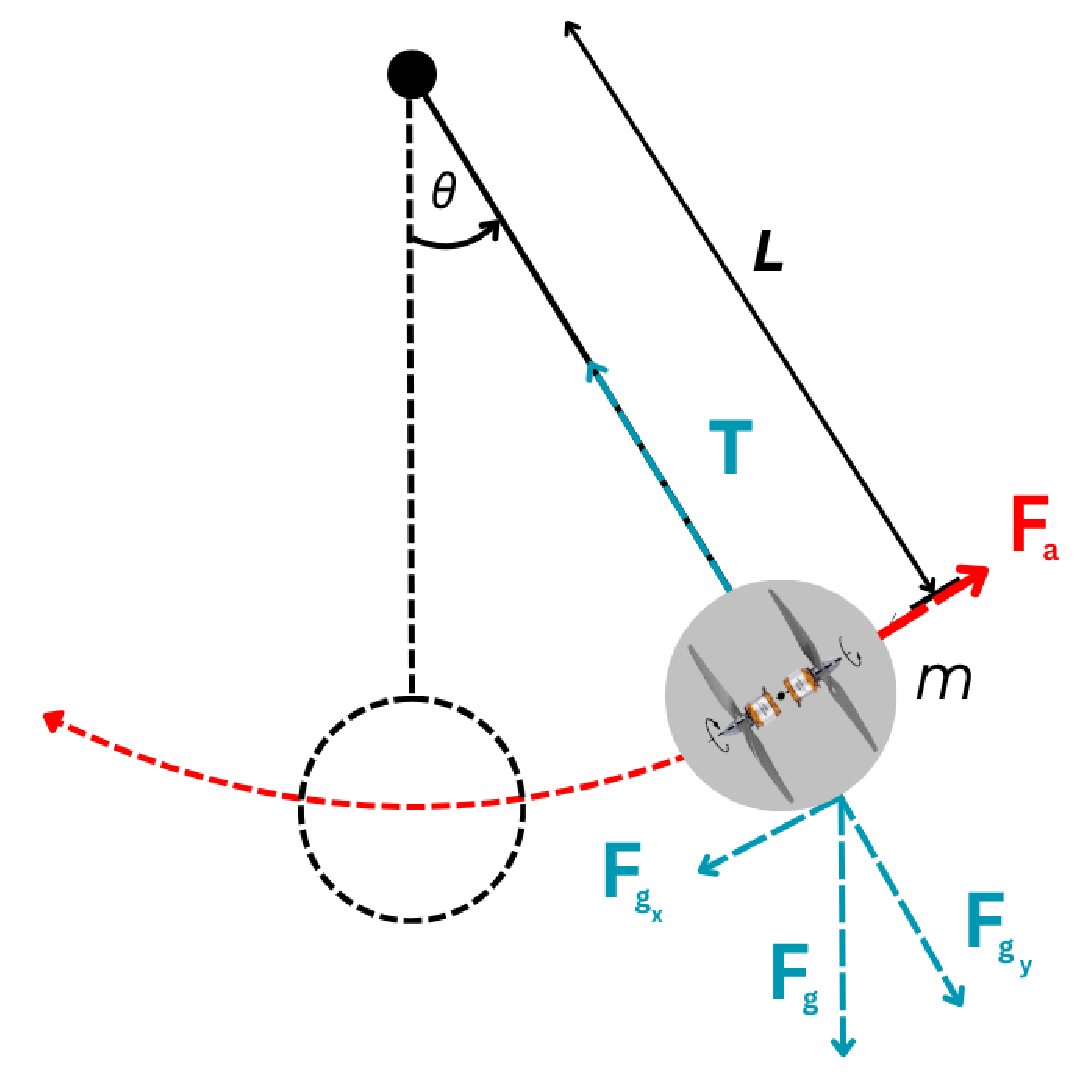
\includegraphics[width=0.35\textwidth]{pendulo-ma.eps}
    \caption{Schematic diagram of the pendulum system.}
    \label{fig:aeropendulum_schematic}
\end{figure}

The structural setup is modeled as a mass $m$ concentrated at the tip of a rigid rod of length $L$, deflected by an angle $\theta$ relative to the vertical equilibrium plane. The gravitational force $F_g = m_{\text{total}}g$ acting on the center of mass is decomposed into two orthogonal components: the radial force $F_{g_{y}} = m_{\text{total}}g\cos\theta$, which acts along the longitudinal axis of the rod and is counterbalanced by the internal structural tension force $T$, and the tangential force $F_{g_{x}} = m_{\text{total}}g\sin\theta$. This tangential component acts perpendicularly to the rod, consistently pulling the system back toward the stable vertical rest position ($\theta = 0^\circ$).

By taking the pivot as the rotational origin and applying the principle of superposition to all coincident perpendicular effects, the dynamic torque balance equation is expressed as:

\begin{equation}
\tau_{m}(t) + \tau_r(t) + \tau_a(t) = I_{\text{total}} \ddot{\theta}(t)
\label{eq:torque_superposition}
\end{equation}

\noindent where $\tau_{m}(t)$ represents the active net propulsive torque generated by the twin-propeller assembly at the tip, defined by the operational difference between the front and rear actuators ($\tau_{m}(t) = \tau_{m1}(t) - \tau_{m2}(t)$). The term $\tau_r(t)$ is the gravitational restoring torque directly derived from the tangential force component shown in the schematic diagram, defined as$\tau_r(t) = -LF_{g_x}= -L m_{\text{total}}g\sin\theta(t)$, where the negative sign denotes its restorative nature opposing the angular displacement. Finally, $\tau_a(t)$ is the non-conservative aerodynamic drag torque that models the atmospheric fluid resistance opposing the motion of the rod through the air, given by:

\begin{equation}
\tau_a(t) = -b \dot{\theta}(t)
\label{eq:damping_torque}
\end{equation}

\noindent where $b$ denotes the rotational viscous damping coefficient and $\dot{\theta}(t)$ represents the instantaneous angular velocity of the plant.

The structural resistance to change in its rotational state, quantified by the total moment of inertia ($I_{\text{total}}$) about the rotation axis, must also be parameterized. This value is determined by combining the continuous mass distribution of the homogeneous rigid rod and the discrete masses of the two actuators located at its tip. Assuming a uniform mass distribution along the rod of length $L$ and mass $m_{\text{haste}}$, and modeling the two BLDC motors as point masses of value $m_{\text{motor}}$ located at a distance $L$ from the pivot, the total equivalent moment of inertia is established via superposition as:

\begin{equation}
I_{\text{total}} = L^2 \left( \frac{1}{3}m_{\text{haste}} + 2m_{\text{motor}} \right)
\label{eq:i_total}
\end{equation}

Once all individual torque components acting on the mechanical structure and the geometric parameters are explicitly defined, they can be directly substituted into the general mechanical balance represented in Eq. \eqref{eq:torque_superposition}. Consequently, the full non-linear second-order ordinary differential equation that governs the twin-rotor aeropendulum dynamic behavior is obtained:

\begin{equation}
\begin{split}
L^{2}\left(\frac{1}{3}m_{\text{haste}}+2m_{\text{motor}}\right)\ddot{\theta}(t) + b\dot{\theta}(t) \\
+ Lm_{\text{total}}g\sin\theta(t) = \tau_{m1}(t) - \tau_{m2}(t)
\end{split}
\label{eq:nonlinear_ode}
\end{equation}

For the development of classical linear control architectures, the non-linear operating region can be linearized around the stable vertical equilibrium position ($\theta = 0^\circ$). Utilizing the small-angle Taylor approximation ($\sin\theta \approx \theta$), the fundamental expression reduces to a linear ordinary differential equation. By assuming that the structural lumped parameters of the passive pendulum can be aggregated, the gravitational torque constant $K_g$ is defined as:

\begin{equation}
K_g = L m_{\text{total}} g
\label{eq:const_Kg}
\end{equation}

\noindent where $m_{\text{total}}$ represents the total mass of the pendulum assembly, $L$ is the distance from the pivot to the center of mass, and $g$ is the acceleration due to gravity. 
Within this context, the simplified representation of the equation can be expressed as in Eq.~\eqref{eq:linear_ode_compact}:

\begin{equation}
I_{\text{total}} \ddot{\theta}(t) + b \dot{\theta}(t) + K_g \theta(t) = \tau_{m1}(t) - \tau_{m2}(t)
\label{eq:linear_ode_compact}
\end{equation}

Assuming zero initial mechanical conditions ($\theta(0) = 0$ and $\dot{\theta}(0) = 0$), the application of the Laplace transform to this model maps the dynamics directly into the complex frequency $s$-domain. Ultimately, the open-loop transfer function $G(s)$, which represents the system's open-loop equation and establishes the dynamic relationship between the net propulsive torque input and the resulting angular position output $\Theta(s)$, is rigorously derived as:

\begin{equation}
G(s) = \frac{\Theta(s)}{T_{m1}(s) - T_{m2}(s)} = \frac{1}{J s^2 + b s + K_g}
\label{eq:transfer_function_compact}
\end{equation}

\section{Experimental platform and parameter identification}

To evaluate the mathematical formulations and validate the proposed control strategies, a dedicated experimental testbed was developed and utilized in this work. The physical apparatus consists of a twin-rotor aeropendulum framework, illustrated in Fig.~\ref{fig:aeropendulum_combined}, designed for the study and benchmark of non-linear control techniques.

\begin{figure}[htbp]
    \centering
    \begin{subfigure}{0.265\textwidth}
        \centering
        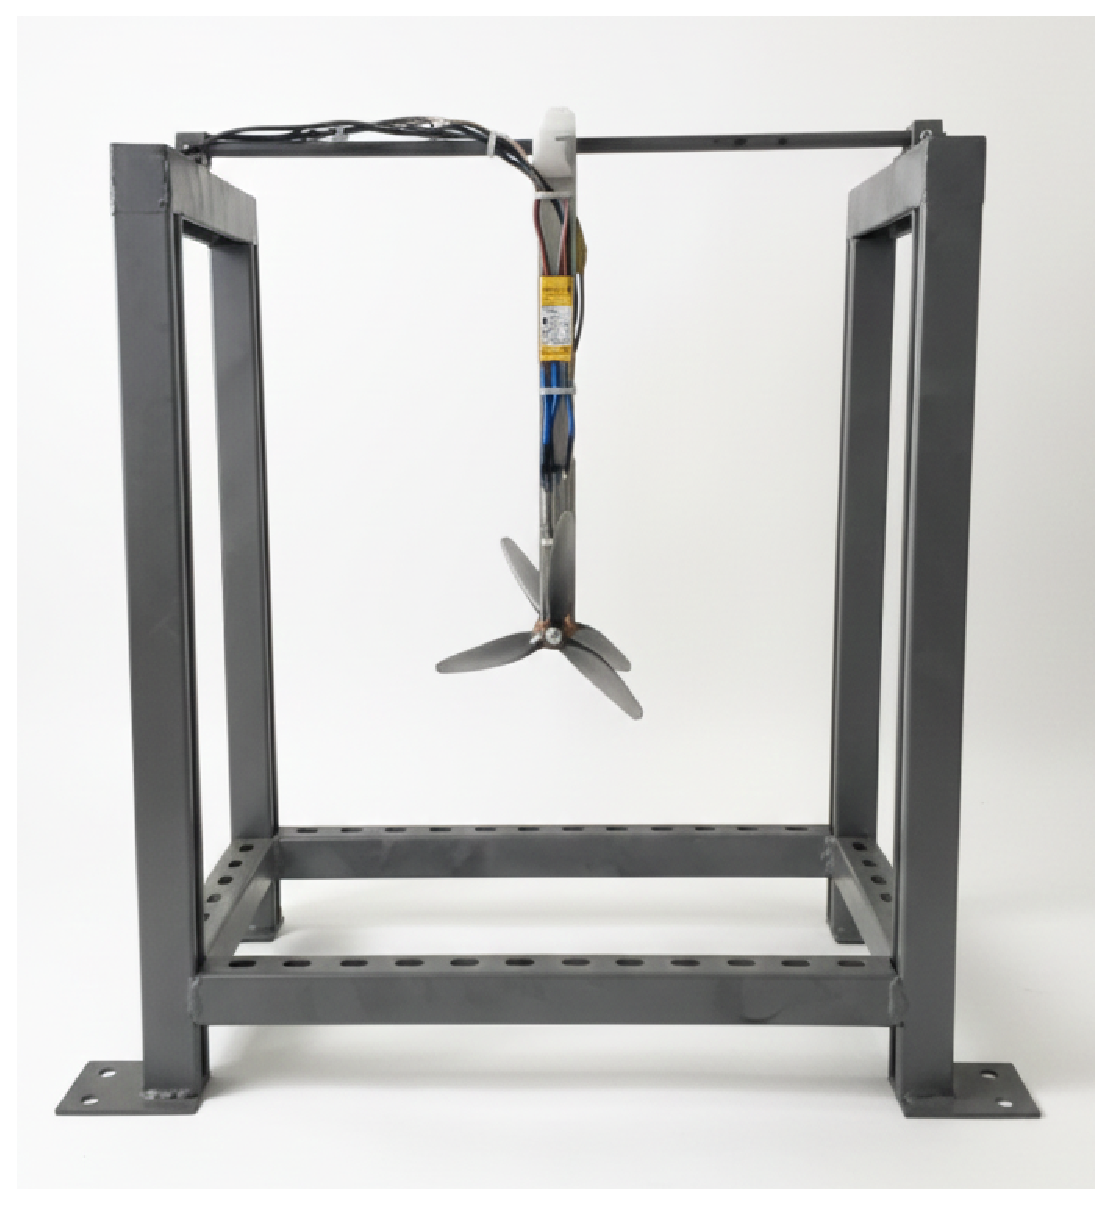
\includegraphics[width=\textwidth]{pendulum-front.eps}
        \caption{Front view.}
        \label{fig:aeropendulum_front}
    \end{subfigure}
    \hfill
    \begin{subfigure}{0.19\textwidth}
        \centering
        \includegraphics[width=\textwidth]{pendulum-lateral.eps}
        \caption{Side view.}
        \label{fig:aeropendulum_side}
    \end{subfigure}
    \caption{The developed twin-rotor aeropendulum experimental platform from front and side perspectives.}
    \label{fig:aeropendulum_combined}
\end{figure}

The mechanical assembly isolates the plant's movement to a single rotational degree of freedom within the vertical plane. The main structural components, geometric constraints, and the instrumentation infrastructure are detailed below.

\subsection{Mechanical and Hardware Architecture}
\label{sub:hardware}

The structural support consists of a rigid frame that holds the primary rotational shaft. To minimize frictional losses and guarantee that the plant dynamics are predominantly driven by the active aerodynamic inputs, the mechanical assembly is coupled to the fixed frame through low-friction bearings. 

The primary physical and operational characteristics of the embedded subsystems are defined as follows:
\begin{itemize}
    \item \textbf{Propulsion Subsystem:} Actuation is provided by two A2212/13T Brushless DC (BLDC) motors mounted back-to-back at the lower tip of a rigid aluminum rod ($L = 0.515\text{ m}$). Each motor is coupled to a $7\times4\times3$ polycarbonate tri-blade propeller. This assembly converts the digital control commands into active differential thrust forces perpendicular to the longitudinal axis of the rod.
    \item \textbf{Processing and Control Unit:} The computational core is driven by an ATmega2560 microcontroller (Arduino Mega platform). This unit is responsible for executing the real-time digital filtering routines, processing the control laws, and generating the independent high-resolution Pulse Width Modulation (PWM) signals dispatched to the Electronic Speed Controllers (ESCs). The control loop runs at a fixed sampling period, and data communication with the host computer is established via a bidirectional USB/Serial interface.
    \item \textbf{Sensors and Interface Subsystems:} The angular position $\theta(t)$ is acquired through a high-precision rotary potentiometer attached directly to the main pivot axis, selected due to its high linearity and noise immunity. 
    \item \textbf{Power Supply Unit:} To ensure voltage stability and satisfy the strict current demands during high-acceleration transients, the entire platform is powered by a regulated $10\text{ V}$, $30\text{ A}$ switched-mode power supply (SMPS).
    \item \textbf{Supervisory and Graphical User Interface (GUI):} A dedicated telemetry and supervisory software system was developed to mediate the experimental verification procedures. Operating over the bidirectional serial communication channel, this graphical interface allows the real-time configuration of setpoints and control parameters while simultaneously logging the estimated variables, sensor measurements, and actuator efforts for post-processing and dynamic analysis.
\end{itemize}

\subsection{System Parameter Identification}
\label{sub:parameters}

Based on the physical construction and geometric synthesis of the prototype, the core structural and dynamic variables of the system were successfully determined. The mass elements and physical lengths were measured directly from the experimental apparatus, while parameters such as the total mass moment of inertia ($I_{\text{total}}$) and the experimental rotational viscous damping coefficient ($b$) were obtained through analytical formulations and free-oscillation dynamic tests, respectively. 

The complete set of identified physical constants and operational parameters that govern the aeropendulum dynamics is consolidated in Table~\ref{tab:system_parameters}.

\begin{table}[h]
\caption{Physical and identified parameters of the developed aeropendulum platform}\label{tab:system_parameters}%
\begin{center}
\begin{minipage}{\columnwidth}
%%\setlength{\tabcolsep}{6pt} % Ajusta o espaçamento entre colunas para o layout
\footnotesize % Fonte padrão aceita pela Springer para tabelas compactas
\begin{tabular*}{\columnwidth}{@{\extracolsep{\fill}}@{}lll@{}}
\toprule
\textbf{Parameter} & \textbf{Value} & \textbf{Unit} \\
\midrule
Motor mass ($m_1 = m_2$) & 0,052 & kg \\
Rod mass ($m_{\text{haste}}$) & 0,100 & kg \\
Total moment of inertia ($I_{\text{total}}$) & 0,0173 & kg$\cdot$m² \\
Viscous damping coefficient ($b$) & 0,3944 & N$\cdot$m$\cdot$s/rad \\
Acceleration of gravity ($g$) & 9,8 & m/s² \\
Rod length ($L$) & 0,36 & m \\
\botrule
\end{tabular*}
\end{minipage}
\end{center}
\end{table}


\section{Input signal interpretation and actuation dynamics}\label{sec3}

In phenomenological modeling, the input is conventionally defined by the pure net aerodynamic torque developed by the propulsion units. However, from a practical control systems perspective, the actuators cannot be directly driven by a torque command. Instead, they must be excited via voltage or current variables. This section establishes the mathematical and experimental formulations for two distinct actuation paradigms: voltage-based equivalent actuation and estimated current-based actuation. These formulations redefine the open-loop plant inputs, establishing the basis for the comparative analysis.

\subsection{Voltage-Based Actuation Dynamics}
\label{sub:voltage_actuation}

The operation of Brushless DC (BLDC) motors relies on the electromagnetic interaction between the stator windings and the permanent magnet rotor. The fundamental torque generation is structurally governed by the motor torque constant ($K_t$), which linearly relates the mechanical torque to the armature current ($i_a$):

\begin{equation}
\tau(t) = K_t i_a(t)
\label{eq:torque_kt}
\end{equation}

\noindent where $K_t$ is the motor torque constant, which is inversely proportional to the motor velocity constant ($K_v$, specified by the manufacturer as $1000\text{ RPM/V}$ for the actuators utilized in this platform) according to the structural relation:

\begin{equation}
K_t = \frac{60}{2\pi K_v} \approx 0,00955 \text{ N}\cdot\text{m/A}
\label{eq:kt_value}
\end{equation}

To establish a direct practical relationship between the applied terminal voltage ($V$) and the resulting torque ($\tau$), this work proposes an experimental characterization based on steady-state equilibrium conditions. Under this framework, we propose that the armature current $i_a(t)$ can be correlated to the structural angular displacement $\theta(t)$ attained by the aeropendulum through an empirical proportionality coefficient $K_{fi}$:

\begin{equation}
i_a(t) = K_{fi} \theta(t)
\label{eq:ia_kfi}
\end{equation}

Concurrently, we propose a secondary linear relationship to link the steady-state angular displacement to the equivalent average terminal voltage ($V(t)$) applied to the Electronic Speed Controllers (ESCs). This correlation is defined by the coefficient $K_{fv}$ as follows:

\begin{equation}
\theta(t) = K_{fv} V(t)
\label{eq:theta_kfv}
\end{equation}

By combining these proposed steady-state relations, the active torque produced by an isolated motor can be coupled to its terminal voltage input through a lumped equivalent voltage-to-torque gain ($K_{\text{equivalent}}$):

By substituting \eqref{eq:theta_kfv} into \eqref{eq:ia_kfi}, and the result into the fundamental torque relation \eqref{eq:torque_kt}, the active torque produced by an isolated motor can be directly coupled to its terminal voltage input through a lumped equivalent voltage-to-torque gain ($K_{\text{equivalent}}$):

\begin{equation}
\tau(t) = K_t K_{fi} K_{fv} V(t) = K_{\text{equivalent}} V(t)
\label{eq:torque_kequiv}
\end{equation}

To parameterize this model for the bidirectional setup, systematic experimental calibration procedures were conducted. Specific Pulse Width Modulation (PWM) duty cycles were applied step-wise to the front and rear actuators. The corresponding armature current, equivalent terminal voltage, and steady-state angular deflections were recorded. 

Linear regression algorithms were applied to the experimental curves, mapping the correlation parameters. The calculated gains $K_{fi}$, $K_{fv}$, and the resulting lumped $K_{\text{equivalent}}$ parameters for both propulsion units are consolidated in Table~\ref{tab:voltage_parameters}.

\begin{table}[h]
\caption{Static calibration parameters for voltage actuation}\label{tab1}%
\begin{center}
\begin{minipage}{\columnwidth}
%%\setlength{\tabcolsep}{4.5pt} % Ajusta o espaço entre colunas nativamente
\footnotesize % Reduz a fonte de forma aceita pela Springer
\begin{tabular*}{\columnwidth}{@{\extracolsep{\fill}}@{}llll@{}}
\toprule
Actuator & $K_{f_i} \text{ (A/}^\circ\text{)}$ & $K_{f_v} \text{ (}^\circ\text{/V)}$ & $K_{\text{equivalent}} \text{ (N}{m/V)}$ \\
\midrule
Front & 0,053252 & 8,26146 & 0,00420 \\
Rear  & -0,121940 & -5,11253 & 0,00595 \\
\botrule
\end{tabular*}
\end{minipage}
\end{center}
\label{tab:voltage_parameters}
\end{table}
Thus, by applying the algebraic difference between the independent actuators, the net voltage-driven propulsive torque command is defined as $\tau_{m1}(t) - \tau_{m2}(t) = K_{\text{equivalent},1}V_1(t) - K_{\text{equivalent},2}V_2(t)$.

\subsection{Current-Based Actuation Dynamics}
\label{sub:current_actuation}

Unlike the voltage paradigm where torque coupling is indirect and relies on multi-stage linear approximations—current-based actuation leverages the direct, uncoupled physical relationship between armature current and torque expressed in Eq. \eqref{eq:torque_kt}. Actuating the plant via current provides a more linear control loop, as it inherently diminishes the back-electromotive force (Back-EMF) variations and armature resistance thermal dependencies.

Since the experimental platform lacks integrated real-time physical current sensors on its embedded hardware, a virtual current sensing loop was developed in software. To establish this sensorless framework, a preliminary steady-state empirical characterization was executed to map the relationship between the applied control variable ($PWM$) and the resulting armature current ($I$). 

Through systematic experimental trials, a mapping was conducted to characterize the relationship between the electrical current consumed and the applied pulse-width modulation (PWM) signal for each propulsion unit. By applying a linear approximation to the gathered experimental steady-state data, this behavior was mathematically modeled as:

\begin{equation}
I(t) = a \cdot PWM(t) + b
\label{eq:pwm_current_linear}
\end{equation}

\noindent where $a$ and $b$ denote the empirical slope and offset coefficients, respectively, obtained through linear regression. The resulting parametric values for each actuator are summarized in Table~\ref{tab:current_parameters}.

\begin{table}[h]
\caption{Identified PWM-to-Current calibration functions}\label{tab:current_parameters}%
\begin{center}
\begin{minipage}{\columnwidth}
\setlength{\tabcolsep}{6pt} % Ajusta o espaço entre colunes nativamente
\footnotesize % Reduz a fonte de forma aceita pela Springer
\begin{tabular*}{\columnwidth}{@{}ll@{}}
\toprule
Actuator &  Function $I(t) = a \cdot \text{PWM}(t) + b$ \\
\midrule
Front & $I_1(t) = 0.006427 \cdot \text{PWM}_1(t) - 7.139481$ \\
Rear  & $I_2(t) = 0.007061 \cdot \text{PWM}_2(t) - 7.643550$ \\
\botrule
\end{tabular*}
\end{minipage}
\end{center}
\end{table}

For the physical embedded implementation, this mapping is inverted inside the processing unit to establish the virtual current loop. The software execution framework processes the demanded reference current ($I_{\text{ref}}$) for each motor and maps it into a corresponding digital command through the following static inversion sequence:

\begin{enumerate}
    \item The algorithm takes the desired current variable, $I_{\text{ref}}(t)$, which acts as the intermediate control input for the actuation subsystem.
    \item The software execution loop applies the analytical inverse of the experimentally identified linear functions to convert this reference current into its corresponding digital $\text{PWM}$ duty cycle:
    \begin{equation}
    \text{PWM}(t) = \frac{I_{\text{ref}}(t) - b}{a}
    \label{eq:inverse_pwm}
    \end{equation}
    \noindent where $a$ and $b$ represent the specific empirical parameters of the respective actuator, as consolidated in Table~\ref{tab:current_parameters}.
    \item The computed duty cycle is directly dispatched to the microprocessor internal timers to synthesize the physical hardware signal that drives the ESCs.
\end{enumerate}

This procedure implements a virtual current loop entirely in software, simulating the behavior of a physical current-driven actuator without the need for real-time sensing infrastructure.

This methodology successfully implements an indirect virtual current loop in software, replicating the performance of a cascaded hardware control topology without requiring real-time physical current sensing infrastructure.



\section{Control system design}\label{sec4}

This work proposes and evaluates two distinct control paradigms to regulate the angular position of the twin-rotor aeropendulum: a classical Proportional-Integral-Derivative (PID) controller and an intelligent hybrid Fuzzy-PID controller. Both architectures are independently implemented and compared under both voltage and virtual current actuation frameworks, mapping the performance boundaries of each combination.

\subsection{Classical PID Control Design and Tuning}
\label{sub:pid_design}

The classical position control loop is structured around a parallel linear PID topology. The synthesis utilizes the open-loop transfer functions derived for current actuation ($G_1(s)$) and voltage actuation ($G_2(s)$), which represent the system's open-loop equations and are expressed as:

\begin{equation}
G_1(s) = \frac{\Theta(s)}{I_{m1}(s) - I_{m2}(s)} = \frac{K_t / I_{\text{total}}}{s^2 + \frac{b}{I_{\text{total}}}s + \frac{K_g}{I_{\text{total}}}}
\label{eq:tf_current_literal}
\end{equation}

\begin{equation}
G_2(s) = \frac{\Theta(s)}{V_1(s) - V_2(s)} = \frac{(K_1 + K_2) / I_{\text{total}}}{s^2 + \frac{b}{I_{\text{total}}}s + \frac{K_g}{I_{\text{total}}}}
\label{eq:tf_voltage_literal}
\end{equation}

The characteristic polynomial of the linearized system yields two distinct, real negative poles. To establish an analytical baseline, the classic open-loop Ziegler–Nichols (ZN) tuning methodology was applied. These initial parameter values, consolidated in Table~\ref{tab:pid_zn_base}, served as the starting baseline configuration evaluated during the preliminary simulation stage.

\begin{table}[h]
\caption{Initial Ziegler–Nichols baseline parameters for the PID controller}\label{tab:pid_zn_base}%
\begin{center}
\begin{minipage}{\columnwidth}
\footnotesize
\begin{tabular*}{\columnwidth}{@{\extracolsep{\fill}}@{}llll@{}}
\toprule
\textbf{Control Framework} & $\mathbf{K_p}$ & $\mathbf{K_i}$ & $\mathbf{K_d}$ \\
\midrule
Voltage Proportional & 1,495 & 2,889 & 0,129 \\
Virtual Current      & 0,641 & 0,155 & 0,664 \\
\botrule
\end{tabular*}
\end{minipage}
\end{center}
\end{table}

\subsection{Adaptive Fuzzy-PID Control Design}
\label{sub:fuzzy_pid}

To enhance tracking robustness against parameter variations and unmodeled non-linear dynamics, an adaptive hybrid Fuzzy-PID controller is synthesized. Unlike classical structures with fixed parameters, the proposed architecture updates the proportional ($K_p$), integral ($K_i$), and derivative ($K_d$) gains in real-time. The block topology uses a Mamdani-type Fuzzy Inference System (FIS) acting as an online tuning mechanism over the nominal parallel baseline gains ($K_{p0}, K_{i0}, K_{d0}$) established in Table~\ref{tab:pid_zn_base}. 

The real-time adaptation mechanism is mathematically governed by three dimensionless multiplicative scaling vectors ($\alpha_p, \alpha_i, \alpha_d$), defined as follows:
\begin{equation}
K_p(t) = \alpha_p(t) \cdot K_{p0}
\label{eq:fuzzy_kp}
\end{equation}
\begin{equation}
K_i(t) = \alpha_i(t) \cdot K_{i0}
\label{eq:fuzzy_ki}
\end{equation}
\begin{equation}
K_d(t) = \alpha_d(t) \cdot K_{d0}
\label{eq:fuzzy_kd}
\end{equation}

The FIS operates via two continuous crisp inputs: the tracking position error $e(t) = \theta_{\text{ref}}(t) - \theta(t)$ and its discrete finite-difference derivative $\dot{e}(t)$. Both input domains are mapped into three linguistic variables: Negativo (N), Zero (Z), and Positivo (P). The internal cross-coupled heuristic knowledge base consists of 9 linguistic IF-THEN rules deduced empirically from simulation behaviors, structured to minimize oscillations while accelerating transient recovery. The unifom rule base is consolidated in Table~\ref{tab:fuzzy_rules}.

\begin{table}[h]
\caption{Heuristic rule base for the adaptive Fuzzy-PID inference system}\label{tab:fuzzy_rules}%
\begin{center}
\begin{minipage}{\columnwidth}
\footnotesize
\begin{tabular*}{\columnwidth}{@{\extracolsep{\fill}}@{}lllll@{}}
\toprule
\textbf{Error ($e$)} & \textbf{Derivative ($\dot{e}$)} & $\mathbf{\alpha_p}$ & $\mathbf{\alpha_i}$ & $\mathbf{\alpha_d}$ \\
\midrule
N & N & Medium & Low & High \\
N & Z & Medium & Medium & Medium \\
N & P & Medium & Low & High \\
\midrule
Z & N & Low & Medium & High \\
Z & Z & Medium & Medium & Medium \\
Z & P & Low & Medium & High \\
\midrule
P & N & Medium & Low & High \\
P & Z & Medium & Medium & Medium \\
P & P & Medium & Low & High \\
\botrule
\end{tabular*}
\vskip 4pt
\scriptsize\textbf{Note:} N: Negative; Z: Zero; P: Positive.
\end{minipage}
\end{center}
\end{table}

To balance computational efficiency and smooth interpolation boundaries across the operational space, four-parameter trapezoidal membership functions $\mu(x) = [x_1, x_2, x_3, x_4]$ are implemented for the output channels. The physical constraints and explicit boundary coordinates assigned to each linguistic output region are summarized in Table~\ref{tab:membership_parameters}.

\begin{table}[h]
\caption{Membership function coordinates for the fuzzy scaling outputs}\label{tab:membership_parameters}
\begin{minipage}{\columnwidth}
\footnotesize
\begin{tabular*}{\columnwidth}{@{\extracolsep{\fill}}@{}llc@{}}
\toprule
\textbf{Output} & \textbf{Region}\footnote{The abbreviations represent the fuzzy linguistic regions: Low (L), Medium (M), Normal (N), and High (H).} & $\mathbf{[x_1;\, x_2;\, x_3;\, x_4]}$ \\
\midrule
                        & L & $[0.10;\, 0.10;\, 0.20;\, 0.30]$ \\
$\alpha_p \in [0;\, 1]$ & M & $[0.20;\, 0.40;\, 0.60;\, 0.80]$ \\
                        & H & $[0.70;\, 0.85;\, 1.00;\, 1.00]$ \\
\midrule
                            & L & $[0.30;\, 0.50;\, 0.60;\, 0.80]$ \\
$\alpha_i \in [0.3;\, 1.5]$ & N & $[0.75;\, 0.82;\, 1.18;\, 1.26]$ \\
                            & H & $[1.18;\, 1.25;\, 1.42;\, 1.50]$ \\
\midrule
                        & L & $[0.095;\, 0.171;\, 0.280;\, 0.370]$ \\
$\alpha_d \in [0;\, 1]$ & M & $[0.370;\, 0.420;\, 0.550;\, 0.640]$ \\
                        & H & $[0.640;\, 0.710;\, 0.820;\, 1.000]$ \\
\bottomrule
\end{tabular*}
\end{minipage}
\end{table}

The aggregated fuzzy outputs are mapped back into crisp real-time correction factors using the standard center-of-gravity defuzzification method. This adaptive structure is seamlessly wrapped around both the equivalent voltage distribution loop and the virtual current loop to compare transient performance bounds under identical physical excitations.

\begin{figure*}[t]
    \centering
    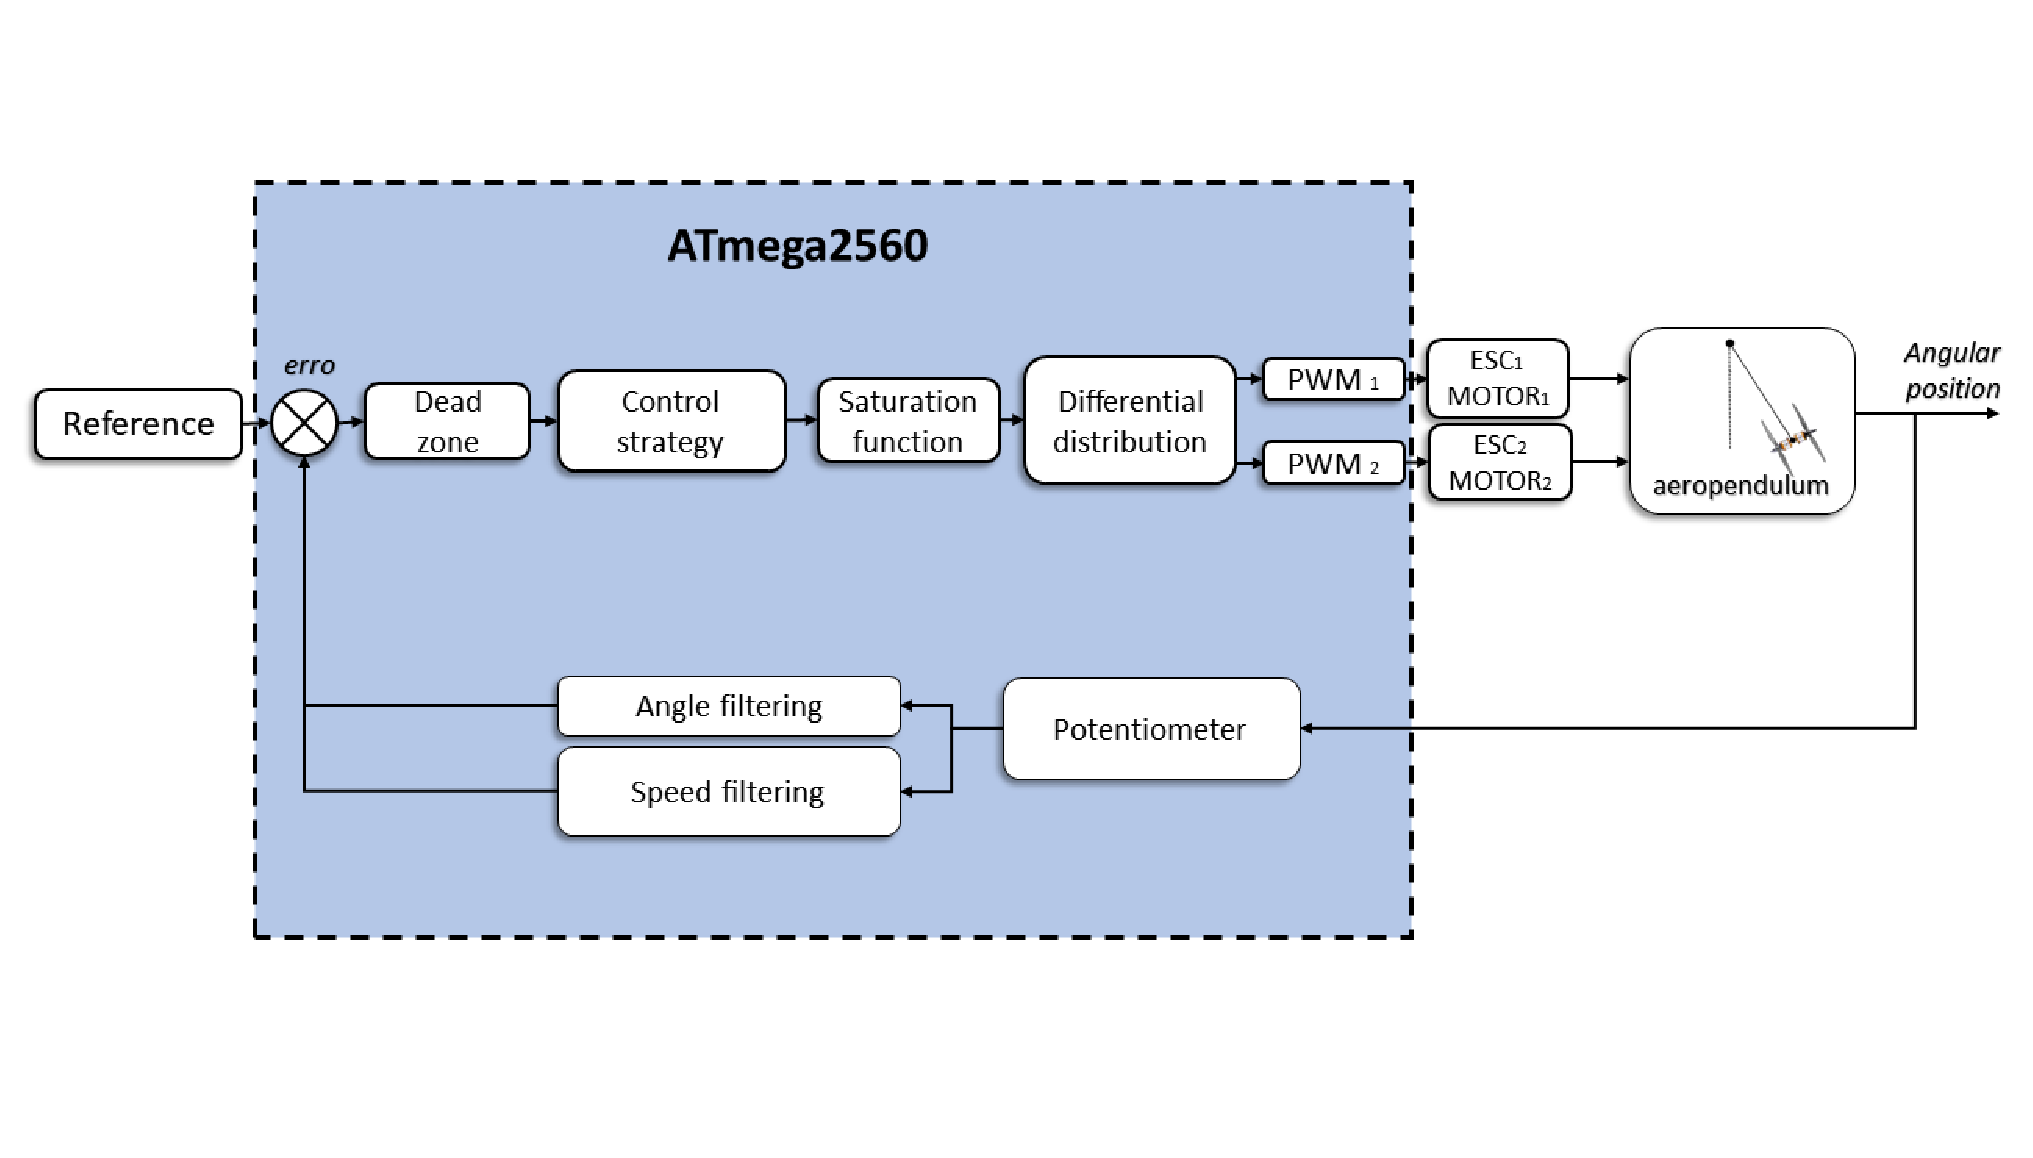
\includegraphics[width=0.9\textwidth]{DiAGRAMAIC_ingles.eps} % O asterisco faz ocupar as duas colunas e o 0.85 expande o tamanho dela na página
    \caption{Real-time signal flow and operational block diagram of the embedded control loop execution.}
    \label{fig:control_flow_diagram}
\end{figure*}

\section{Experimental Results and Discussion}
\label{sec:experimental_results}

This section presents the experimental performance analysis of the twin-rotor aeropendulum under four distinct operational conditions angular step references, evaluated both with and without external disturbances. In each scenario, the classical parallel PID and the adaptive hybrid Fuzzy-PID controllers are comprehensively benchmarked under both equivalent voltage and virtual current actuation frameworks. 

\subsection{Experimental Parameters and Signal Flow Architecture}
\label{sub:experimental_parameters}

The baseline parameters obtained during the simulation stage served as the initial state for the physical embedded system. However, during real-time deployment, minor empirical adjustments were required to compensate for physical motor asymmetries, structural measurement noise, and aerodynamic non-linearities. 

The discrepancy between simulation and experimental parameters is primarily attributed to the current actuation framework. While the analytical model considers the armature current directly via the torque constant ($K_t$), the physical microprocessor outputs a digital $\text{PWM}$ duty cycle proportional to the estimated variable. To bridge this gap and coordinate the physical experiments, a unified execution architecture was developed within the processing unit. The operational signal flow governing this real-time implementation is mapped in Fig.~\ref{fig:control_flow_diagram}.


The finalized controller parameters utilized throughout the experimental campaign are consolidated in Table~\ref{tab:experimental_gains}. The heuristic fuzzy rules and output boundaries established in Section 3 remained unaltered, with gain tuning managed in real-time via the developed supervisory graphical user interface.
\begin{table}[h]
\caption{Final controller parameters applied during the experimental verification}\label{tab:experimental_gains}%
\begin{center}
\begin{minipage}{\columnwidth}
\footnotesize % Fonte padrão aceita pela Springer para tabelas compactas
%
% Usamos tabular* com a largura da coluna e o espaçador automático para encaixe perfeito
\begin{tabular*}{\columnwidth}{@{\extracolsep{\fill}}@{}llll@{}}
\toprule
\textbf{Controller Architecture} & $\mathbf{K_p}$ & $\mathbf{K_i}$ & $\mathbf{K_d}$ \\
\midrule
PID -- Voltage Framework          & 5,00 & 10,00 & 0,200 \\
PID -- Virtual Current Framework  & 0,05 & 0,03  & 0,009 \\
\botrule
\end{tabular*}
\vskip 3pt
\scriptsize\textbf{Note:} Base Fuzzy-PID scaling parameters equal the conventional PID gains.
\end{minipage}
\end{center}
\end{table}


\subsection{Transient Tracking under Step References ($\pm20^\circ$)}
\label{sub:step_tracking}


To evaluate the tracking capability and operational symmetry of the architectures, a $\pm20^\circ$ step reference was commanded at $t = 10\text{ s}$ from a steady state of repose. The resulting angular displacement trajectory is illustrated in Fig.~\ref{fig:angular_displacement_response}, while the corresponding control efforts are shown in Fig.~\ref{fig:control_signals_response}. Additionally, Table~\ref{parametros} provides a quantitative comparison of the time-domain performance metrics, steady-state errors, integrated error indices (IAE, ISE, ITAE), and cumulative control efforts (ISSC).

\begin{figure}[htbp]
    \centering
    \begin{subfigure}{0.4\textwidth}
        \centering
        \includegraphics[width=\textwidth]{posicao_positivo_ingles.eps} % Substitua pelo seu arquivo de +20°
        \caption{Positive step reference ($+20^\circ$).}
        \label{fig:pos_step_20}
    \end{subfigure}
    \\ \vspace{0.2cm} % Quebra a linha para empilhar e adiciona um pequeno espaço vertical elegante
    \begin{subfigure}{0.4\textwidth}
        \centering
        \includegraphics[width=\textwidth]{posicao_negativo_ingles.eps} % Substitua pelo seu arquivo de -20°
        \caption{Negative step reference ($-20^\circ$).}
        \label{fig:neg_step_20}
    \end{subfigure}
    \caption{Experimental tracking under step references.}
    \label{fig:angular_displacement_response}
\end{figure}

\begin{figure}[htbp]
    \centering
    \begin{subfigure}{0.5\textwidth}
        \centering
        \includegraphics[width=\textwidth]{sinal_controle_positivo_ingles.eps} % Substitua pelo nome do arquivo da sua Figura 42
        \caption{Positive step ($+20^\circ$).}
        \label{fig:control_sig_pos}
    \end{subfigure}
    \hfill
    \begin{subfigure}{0.5\textwidth}
        \centering
        \includegraphics[width=\textwidth]{sinal_controle_negativo_ingles.eps} % Substitua pelo nome do arquivo da sua Figura 43
        \caption{Negative step ($-20^\circ$).}
        \label{fig:control_sig_neg}
    \end{subfigure}
    \caption{Real-time control effort signals dispatched to the propulsion units under step references.}
    \label{fig:control_signals_response}
\end{figure}

\begin{table*}[t]
\caption{Combined transient performance metrics, integrated error indices, and energetic control efforts under step references}\label{tab:performance_metrics_combined}%
\begin{center}
\begin{minipage}{\textwidth}
\scriptsize % Tamanho ideal para tabelas densas de 11 colunas
\setlength{\tabcolsep}{3pt} % Espaçamento horizontal elegante para 11 colunas
% Definimos as 11 colunas da tabela: 3 de configuração + 4 métricas temporais/precisão + 4 índices integrais
\begin{tabular*}{\textwidth}{@{\extracolsep{\fill}}@{}lllcccccccc@{}}
\toprule
% Primeira camada do cabeçalho agrupando as métricas por categoria conceitual
\textbf{Setpoint} & \textbf{Actuation} & \textbf{Controller} & \multicolumn{4}{c}{\textbf{Temporal metrics}} & \multicolumn{4}{c}{\textbf{Integral Indices}} \\
\cmidrule(lr){4-7} \cmidrule(lr){8-11}
% Segunda camada com os identificadores específicos de cada coluna
& & & $\mathbf{M_p\,(\%)}$ & $\mathbf{t_r\,(\text{s})}$ & $\mathbf{t_s\,(\text{s})}$ & $\mathbf{e_{\text{ss}}\,(^{\circ})}$ & \textbf{IAE} & \textbf{ISE} & \textbf{ITAE} & \textbf{ISSC} \\
\midrule
            & Voltage  & PID       & 0,50 & 4,78 & 37,39 & 0,10 & 66,05  & 746,64  & 940,03  & 1571,73 \\
$+20^{\circ}$ & Voltage  & Fuzzy-PID & 1,67 & 6,77 & 55,02 & 1,34 & 134,32 & 1263,10 & 2957,58 & 1966,19 \\
            & Current  & PID       & 1,90 & 6,10 & 18,54 & 0,40 & 79,83  & 845,22  & 1214,70 & 624,77  \\
            & Current  & Fuzzy-PID & 2,67 & 8,76 & 50,07 & 0,49 & 114,67 & 1104,99 & 2089,93 & 663,74  \\
\midrule
            & Voltage  & PID       & 2,78 & 4,51 & 54,83 & 0,33 & 69,79  & 726,48  & 1288,53 & 2040,42 \\
$-20^{\circ}$ & Voltage  & Fuzzy-PID & 2,51 & 7,66 & 53,74 & 1,46 & 127,79 & 1201,39 & 2851,11 & 1758,59 \\
            & Current  & PID       & 2,23 & 7,25 & 40,96 & 0,50 & 81,82  & 705,85  & 1407,05 & 508,89  \\
            & Current  & Fuzzy-PID & 1,71 & 9,30 & 25,06 & 0,64 & 118,34 & 1070,72 & 2358,39 & 775,60  \\
\botrule
\label{parametros}
\end{tabular*}
\end{minipage}
\end{center}
\end{table*}

\subsection{Disturbance Rejection under Step References ($\pm20^\circ$)}
\label{sub:disturbance_rejection}

\begin{table*}[t]
\caption{Combined transient performance metrics, integrated error indices, and energetic control efforts under external disturbance}\label{tab:performance_metrics_disturbance}%
\begin{center}
\begin{minipage}{\textwidth}
\scriptsize % Tamanho ideal para tabelas densas
\setlength{\tabcolsep}{4pt} % Aumentamos um pouco o espaçamento já que a tabela tem menos colunas
% Definimos as 11 colunas da tabela: 3 de configuração + 4 métricas temporais/precisão + 4 índices integrais
\begin{tabular*}{\textwidth}{@{\extracolsep{\fill}}@{}lllcccccccc@{}}
\toprule
% Primeira camada do cabeçalho agrupando as métricas por categoria conceitual
\textbf{Setpoint} & \textbf{Actuation} & \textbf{Controller} & \multicolumn{4}{c}{\textbf{Temporal metrics}} & \multicolumn{4}{c}{\textbf{Integral Indices}} \\
\cmidrule(lr){4-7} \cmidrule(lr){8-11}
% Segunda camada com os identificadores específicos de cada coluna
& & & $\mathbf{M_p\,(\%)}$ & $\mathbf{t_r\,(\text{s})}$ & $\mathbf{t_s\,(\text{s})}$ & $\mathbf{e_{\text{ss}}\,(^{\circ})}$ & \textbf{IAE} & \textbf{ISE} & \textbf{ITAE} & \textbf{ISSC} \\
\midrule
            & Voltage  & PID       & 11,32 & 6,01  & 34,78 & 0,50 & 83,34  & 860,66  & 1361,15 & 1077,17 \\
$+20^{\circ}$ & Voltage  & Fuzzy-PID & 6,25  & 6,13  & 34,91 & 0,44 & 95,43  & 1014,02 & 1540,62 & 1229,09 \\
            & Current  & PID       & 4,80  & 10,55 & 31,46 & 0,17 & 121,95 & 1312,82 & 1787,31 & 420,18  \\
            & Current  & Fuzzy-PID & 3,85  & 7,60  & 28,37 & 0,34 & 86,59  & 790,55  & 1293,62 & 387,40  \\
\midrule
            & Voltage  & PID       & 0,41  & 8,62  & 33,33 & 1,31 & 95,07  & 930,59  & 1714,04 & 927,79  \\
$-20^{\circ}$ & Voltage  & Fuzzy-PID & 3,77  & 7,35  & 38,23 & 1,00 & 112,51 & 1111,36 & 2138,56 & 1152,40 \\
            & Current  & PID       & 0,50  & 12,79 & 33,08 & 0,23 & 117,62 & 1013,72 & 1862,83 & 283,40  \\
            & Current  & Fuzzy-PID & 1,62  & 10,42 & 31,05 & 0,36 & 131,05 & 1297,67 & 2346,54 & 597,79  \\
\botrule
\end{tabular*}
\end{minipage}
\end{center}
\end{table*}

The system's resilience and recovery capability were tested by introducing an external physical disturbance after the aeropendulum reached its steady-state operating point. The dynamic angular response under this perturbed condition is captured in Fig.~\ref{fig:disturbance_response}, whereas the control signals dispatched during the stabilization process are detailed in Fig.~\ref{fig:disturbance_control_signals}. To validate these transient behaviors, Table~\ref{tab:performance_metrics_disturbance} consolidates the perturbed performance metrics, error indices, and energetic control expenditures (ISSC).

\begin{figure}[h]
    \centering
    \begin{subfigure}{0.45\textwidth}
        \centering
        \includegraphics[width=\textwidth]{posicao_positivo_disturbio_ingles.eps}
        \caption{Positive step reference ($+20^\circ$) under external disturbance.}
        \label{fig:pos_step_20_dist}
    \end{subfigure}
    \\ \vspace{0.3cm} 
    \begin{subfigure}{0.45\textwidth}
        \centering
        \includegraphics[width=\textwidth]{posicao_negativo_disturbio_ingles.eps}
        \caption{Negative step reference ($-20^\circ$) under external disturbance.}
        \label{fig:neg_step_20_dist}
    \end{subfigure}
    \caption{Experimental angular displacement tracking performance under positive and negative step references with external disturbances.}
    \label{fig:disturbance_response}
\end{figure}

\begin{figure}[h]
    \centering
    \begin{subfigure}{0.5\textwidth}
        \centering
        \includegraphics[width=\textwidth]{sinal_controle_positivo_disturbio_ingles.eps}
        \caption{Control effort during positive step ($+20^\circ$) disturbance recovery.}
        \label{fig:control_sig_pos_dist}
    \end{subfigure}
    \hfill
    \begin{subfigure}{0.5\textwidth}
        \centering
        \includegraphics[width=\textwidth]{sinal_controle_negativo_disturbio_ingles.eps}
        \caption{Control effort during negative step ($-20^\circ$) disturbance recovery.}
        \label{fig:control_sig_neg_dist}
    \end{subfigure}
    \caption{Real-time control effort signals dispatched to the propulsion units during disturbance rejection and recovery.}
    \label{fig:disturbance_control_signals}
\end{figure}


\subsection{Comparative Analysis and Discussion}
\label{sub:comparative_discussion}

The experimental evaluation exposes dynamic and energetic distinctions between the equivalent voltage and estimated current actuation frameworks across both reference directions, under both nominal tracking and perturbed conditions.

\subsubsection{Nominal Step Reference Response}


Under disturbance-free step tracking, the voltage-driven PID controller consistently achieved the fastest initial acceleration, yielding the shortest rise times across both reference directions with minimal overshoot and steady-state error. This responsive behavior indicates a faster initial dynamic response associated with direct voltage actuation. However, this rapid start demands severe actuator aggression, resulting in the highest control efforts observed in the entire nominal test. This high energetic activity indicates a more aggressive control action that imposes significant physical demands on the motor-ESC propulsion modules.

Conversely, the estimated current loop smooths this initial transient. Although it introduces slightly longer rise times, this framework dramatically optimizes the settling time, most notably for the positive step reference. Concurrently, the electrical stress is drastically attenuated, resulting in a substantial reduction in control energy expenditure. This phenomenon confirms the primary advantage of the current-driven paradigm: by embedding the linear current-to-torque relationship directly within the control software, the system successfully minimizes the non-linearities, saturation effects, and thrust asymmetries typical of commercial propulsion units.

The advantages of the proposed virtual current loop become even more prominent when paired with the intelligent Fuzzy-PID controller. For the positive step trajectory, shifting from voltage to current actuation causes a drop in all integrated performance and error indices. A similar behavior is observed for the negative step reference, where the current-loop cascade mapping significantly reduces the settling time while slashing the overall energetic effort. These results demonstrate that combining fuzzy logic with a current-driven framework provides a more damped, highly stable, and energy-efficient dynamic response.

\subsubsection{External Disturbance Rejection and Robustness}
When subjected to external physical disturbances, the current-driven loop demonstrates superior robustness and predictability over the voltage-driven framework, which suffered from high sensitivity and excessive control effort. Under voltage actuation at the positive step reference, the conventional PID reached the highest overshoot of the entire study. Although the Fuzzy-PID controller successfully mitigated this peak, it suffered from degraded integral error indices and a prolonged settling time. 

In contrast, the estimated current loop significantly fortified the system against external impacts. For the positive operating point, the current-driven PID achieved a lower overshoot, a faster settling time, and excellent steady-state precision, while drastically slashing the control effort compared to its voltage counterpart. The absolute best overall performance at this setpoint was achieved by the current-driven Fuzzy-PID, which successfully paired exceptionally low integral error indices with the minimum energetic footprint among all tested configurations, representing superior disturbance rejection and high energy efficiency.

For the negative reference, however, a distinct performance boundary was observed. Here, the current-driven conventional PID achieved the most balanced response, yielding a minimized overshoot, outstanding steady-state accuracy, and the absolute lowest global control effort of all disturbance trials. Conversely, the current-driven Fuzzy-PID experienced a noticeable performance degradation, characterized by a consistent rise in both the integrated error criteria and the energetic effort, alongside a significant increase in the steady-state error. This behavior suggests that for this specific operating zone, the membership functions or rule base of the fuzzy inference system were sub-optimal, leading to control degradation compared to the simpler, conventional PID.


\section{Conclusion}\label{sec5}

This paper presented the development of a compact aeropendulum testbed to experimentally evaluate the impact of low-level actuation on aerospace control systems. The primary contribution consisted in comparing a conventional equivalent voltage-driven scheme against a virtual estimated current-loop, under both classical PID and hybrid Fuzzy-PID control.

The nominal experimental trials demonstrated that the proposed virtual current loop successfully linearizes the actuation channel, mitigating the non-linearities and thrust asymmetries characteristic of commercial motor-ESC propulsion units. When subjected to external disturbances, this current-driven paradigm proved robust, maintaining outstanding steady-state precision while drastically reducing control effort. Although the current-driven Fuzzy-PID scheme established the optimal performance-to-energy trade-off at positive operating points, a distinct operational boundary was observed at negative setpoints; in this latter regime, the conventional PID coupled with virtual current actuation emerged as the most balanced and reliable strategy.


\backmatter

\bmhead{Supplementary information}


\bmhead{Acknowledgements}

?

\section*{Declarations}

Some journals require declarations to be submitted in a standardised format. Please check the Instructions for Authors of the journal to which you are submitting to see if you need to complete this section. If yes, your manuscript must contain the following sections under the heading `Declarations':

\begin{itemize}
\item Funding
\item Conflict of interest/Competing interests (check journal-specific guidelines for which heading to use)
\item Ethics approval and consent to participate
\item Consent for publication
\item Data availability 
\item Materials availability
\item Code availability 
\item Author contribution
\end{itemize}

\noindent
If any of the sections are not relevant to your manuscript, please include the heading and write `Not applicable' for that section. 

%%===================================================%%
%% For presentation purpose, we have included        %%
%% \bigskip command. Please ignore this.             %%
%%===================================================%%
\bigskip
\begin{flushleft}%
Editorial Policies for:

\bigskip\noindent
Springer journals and proceedings: \url{https://www.springer.com/gp/editorial-policies}

\bigskip\noindent
Nature Portfolio journals: \url{https://www.nature.com/nature-research/editorial-policies}

\bigskip\noindent
\textit{Scientific Reports}: \url{https://www.nature.com/srep/journal-policies/editorial-policies}

\bigskip\noindent
BMC journals: \url{https://www.biomedcentral.com/getpublished/editorial-policies}
\end{flushleft}

%%\begin{appendices}

%%\\section{Section title of first appendix}\label{secA1}

An appendix contains supplementary information that is not an essential part of the text itself but which may be helpful in providing a more comprehensive understanding of the research problem or it is information that is too cumbersome to be included in the body of the paper.

%%=============================================%%
%% For submissions to Nature Portfolio Journals %%
%% please use the heading ``Extended Data''.   %%
%%=============================================%%

%%=============================================================%%
%% Sample for another appendix section			       %%
%%=============================================================%%

%% \section{Example of another appendix section}\label{secA2}%
%% Appendices may be used for helpful, supporting or essential material that would otherwise 
%% clutter, break up or be distracting to the text. Appendices can consist of sections, figures, 
%% tables and equations etc.

%%\\end{appendices}

%%===========================================================================================%%
%% If you are submitting to one of the Nature Portfolio journals, using the eJP submission   %%
%% system, please include the references within the manuscript file itself. You may do this  %%
%% by copying the reference list from your .bbl file, paste it into the main manuscript .tex %%
%% file, and delete the associated \verb+\bibliography+ commands.                            %%
%%===========================================================================================%%

\bibliography{sn-bibliography}% common bib file
%% if required, the content of .bbl file can be included here once bbl is generated
%%\input sn-article.bbl

\end{document}
